\subsection{Optimization against Latency}

\subsubsection{Enhancing a Single AXI Transfer}

By increasing the \texttt{TDATA} width, we can accomodate more data in a single AXI transfer\footnote{
    \href{https://developer.arm.com/documentation/ihi0051/a/Introduction/About-the-AXI4-Stream-protocol/Stream-terms}{Stream terms}
}.
The width in the default design is 64 bits, which took 32 cycles to transfer a single input of 256 bytes.
By widening the \texttt{TDATA} width to 256 bits, it takes only 8 cycles to transfer the 256 bytes (\autoref{tab:tdata}).

\begin{table}[ht!]
    \centering
    \caption{\texttt{LOAD\_INPUT} latency under different \texttt{TDATA} width}
    \label{tab:tdata}
    \begin{tabular}{cccccccc}
        \toprule
        \texttt{TDATA} width (bits) & Latency (cycles) & Iteration Latency & Initiation Interval (achieved) & Trip Count & Pipelined \\
        \midrule
        64                          & 4096             & 32                & 32                             & 128        & yes       \\
        128                         & 2048             & 16                & 16                             & 128        & yes       \\
        256                         & 1024             & 8                 & 8                              & 128        & yes       \\
        \bottomrule
    \end{tabular}
\end{table}

\subsubsection{Reducing the Input Dimension}

The size of input is determined by the dimension of inputs (originally \(16 \times 16\)) and the depth of each pixel (8-bit in the previous design).
Reducing the dimension and depth will reduce the amount of transfer and computation.

A search is done by trying different pair of input dimension and depth and calculating the prediction accuracy using the linear model, which is actually a lower bound we can achieve.
The result is as \autoref{fig:mnist-shrink}.
With the input size shrunk to \(8 \times 8\), and the input depth reduced 4 bits,
the prediction accuracy is reduced to 82.96\%, which is worse than our target (over 85\% in accuracy).
However, this is a desirable configuration, which means we can fit an input (64 4-bit pixels) in precisely 32 bytes.
Thus I believe it is worth sacrificing some accuracy here and getting it back using a more aggressive model.

\begin{figure}[ht!]
    \centering
    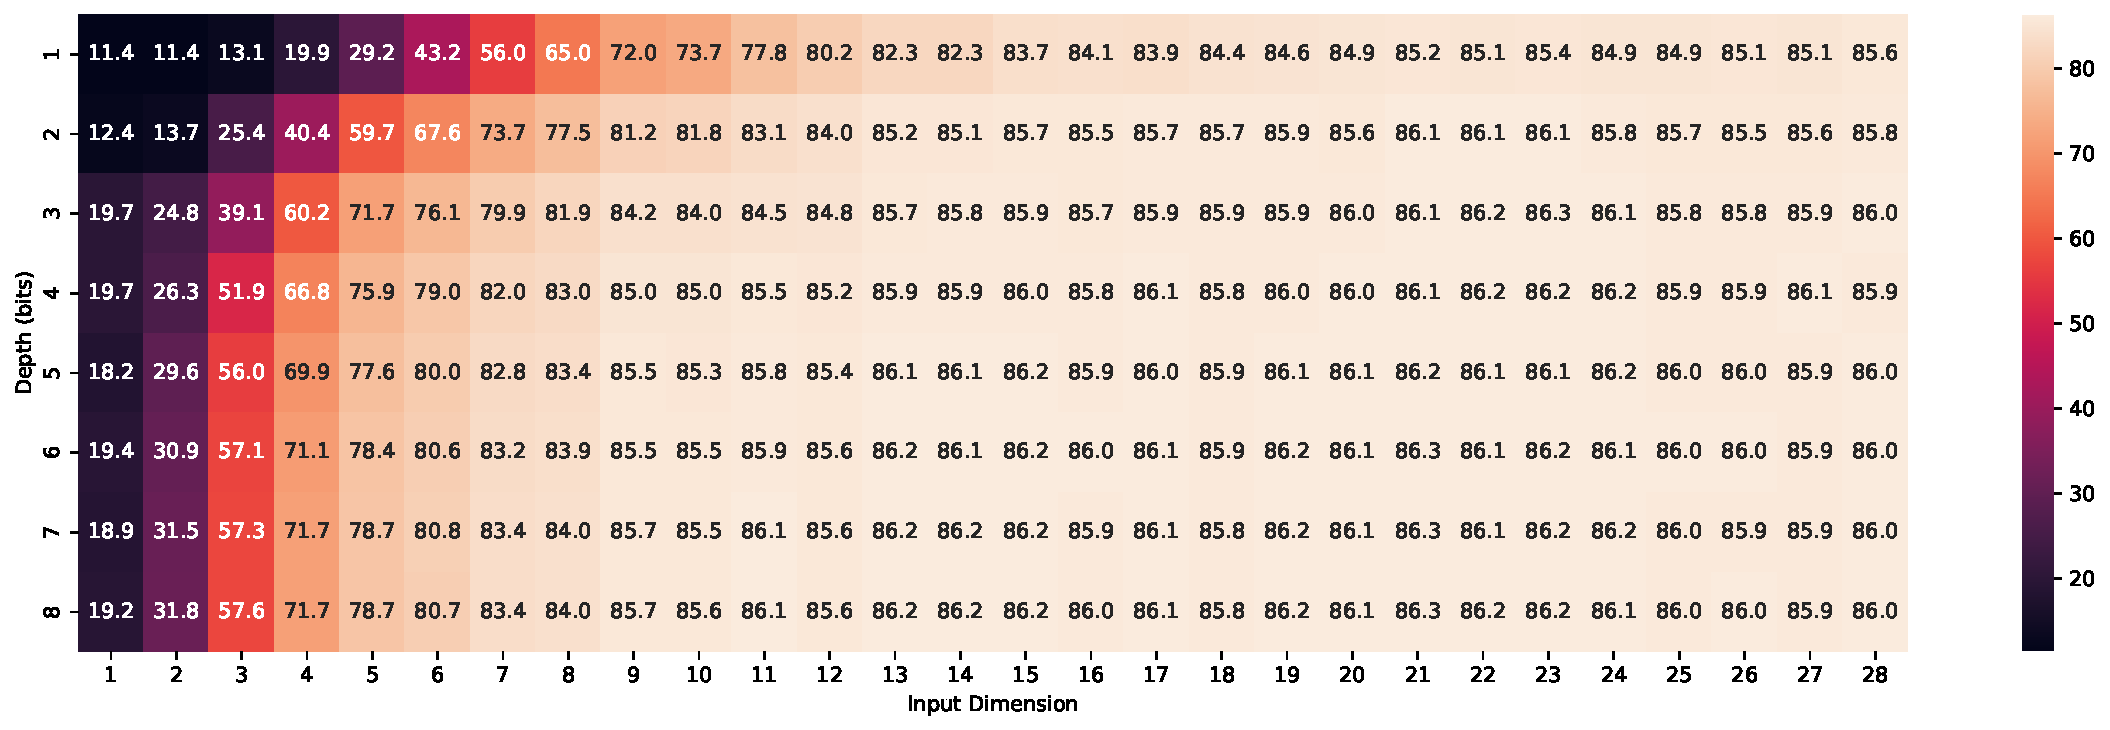
\includegraphics[width=\textwidth]{images/mnist-shrink.pdf}
    \caption{Accuracy of prediction using floating point numbers under different input size}
    \label{fig:mnist-shrink}
\end{figure}

\subsection{Optimization against Accuracy}

The accuracy is improved by using a more complex model, which includes a ReLU activated unbiased input layer (\(64 \times 16\)) and a biased output layer (\(16\times 10\)).
Using ReLU with an unbiased input layer, we can keep the linear property of the model.
That enables us to inherit the methodology applied in \autoref{sec:fixed} to refrain from the floating-point calculation.

\[
    \mathbf{O} = \operatorname{ReLU}(\mathbf{I} \cdot \mathbf{W_1}) \cdot \mathbf{W_2} + \mathbf{b}
\]

After the model, we add a Softmax layer to get a better training result.
This layer can be removed when making predictions on FPGA, which will not affect the final result.
This model achieves a prediction accuracy of 89.88\% using floating-point numbers.

\subsection{Evaluation}

\subsubsection{IP Design}

The overall latency of our design is 159646 cycles, as reported in \autoref{tab:custom-latency}.
Its utilization is as \autoref{tab:w256}.

\begin{table}[ht!]
    \centering
    \caption{Performance Estimates with 256-bit AXI Stream}\label{tab:custom-latency}
    \begin{tabular}{ccccccc}
        \toprule
        \multicolumn{2}{c}{Latency (cycles) }   &
        \multicolumn{2}{c}{Latency (absolute) } &
        \multicolumn{2}{c}{Interval }           &
        \multirow{2}{*}{\makecell*{Pipeline                                                             \\ Type}}                 \\
        min                                     & max    & min      & max      & min    & max    &      \\
        \midrule
        159646                                  & 159646 & 1.596 ms & 1.596 ms & 159647 & 159647 & none \\
        \bottomrule
    \end{tabular}
\end{table}

\begin{table}[ht!]
    \centering
    \caption{Utilization Summary with 256-bit AXI Stream}\label{tab:w256}
    \begin{tabular}{cccccc}
        \toprule
        Name             & BRAM\_18K & DSP & FF     & LUT   & URAM \\
        \midrule
        DSP              & -         & 192 & -      & -     & -    \\
        Expression       & -         & -   & 0      & 4703  & -    \\
        FIFO             & -         & -   & -      & -     & -    \\
        Instance         & 0         & 0   & 36     & 1352  & -    \\
        Memory           & 202       & -   & 32     & 3     & -    \\
        Multiplexer      & -         & -   & -      & 3577  & -    \\
        Register         & -         & -   & 6552   & 128   & -    \\
        \midrule
        Total            & 202       & 192 & 6620   & 9763  & 0    \\
        \midrule
        Available        & 280       & 220 & 106400 & 53200 & 0    \\
        \midrule
        Utilization (\%) & 72        & 87  & 6      & 18    & 0    \\
        \bottomrule
    \end{tabular}
\end{table}

\subsubsection{System Design}

Due to our change of the AXI data width, the MM2S connection between DMA0 and our accelerator module will have a bus interface property mismatch, where the DMA0 provides a 64-bit TDATA bus while mmult\_hw accepts a 256-bit bus.
Thus wee ned to fix the data width of DMA0 manually as \autoref{fig:adjust-axi-data-width}.


\begin{figure}[ht!]
    \centering
    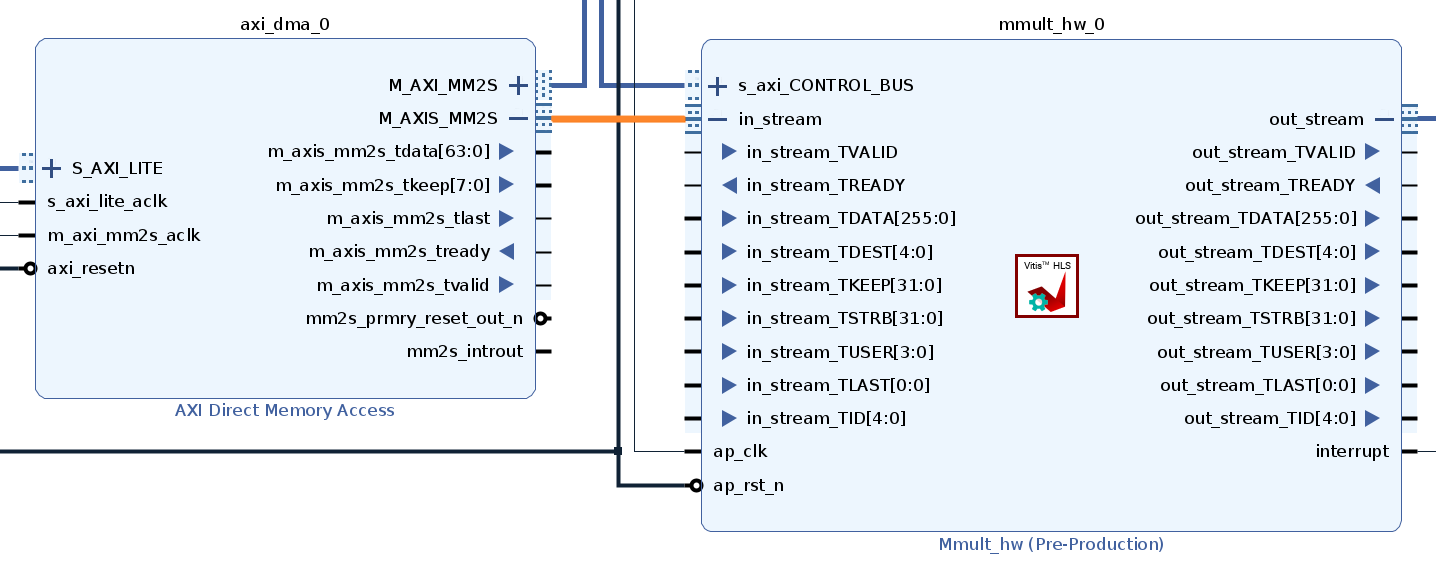
\includegraphics[scale=0.32]{images/tdata-mismatch.png}
    \caption{Bus Interface property \texttt{TDATA\_NUM\_BYTES} does not match}
\end{figure}

\begin{figure}[ht!]
    \centering
    \caption{Adjust AXI data width by re-customizing DMA0}
    \label{fig:adjust-axi-data-width}
    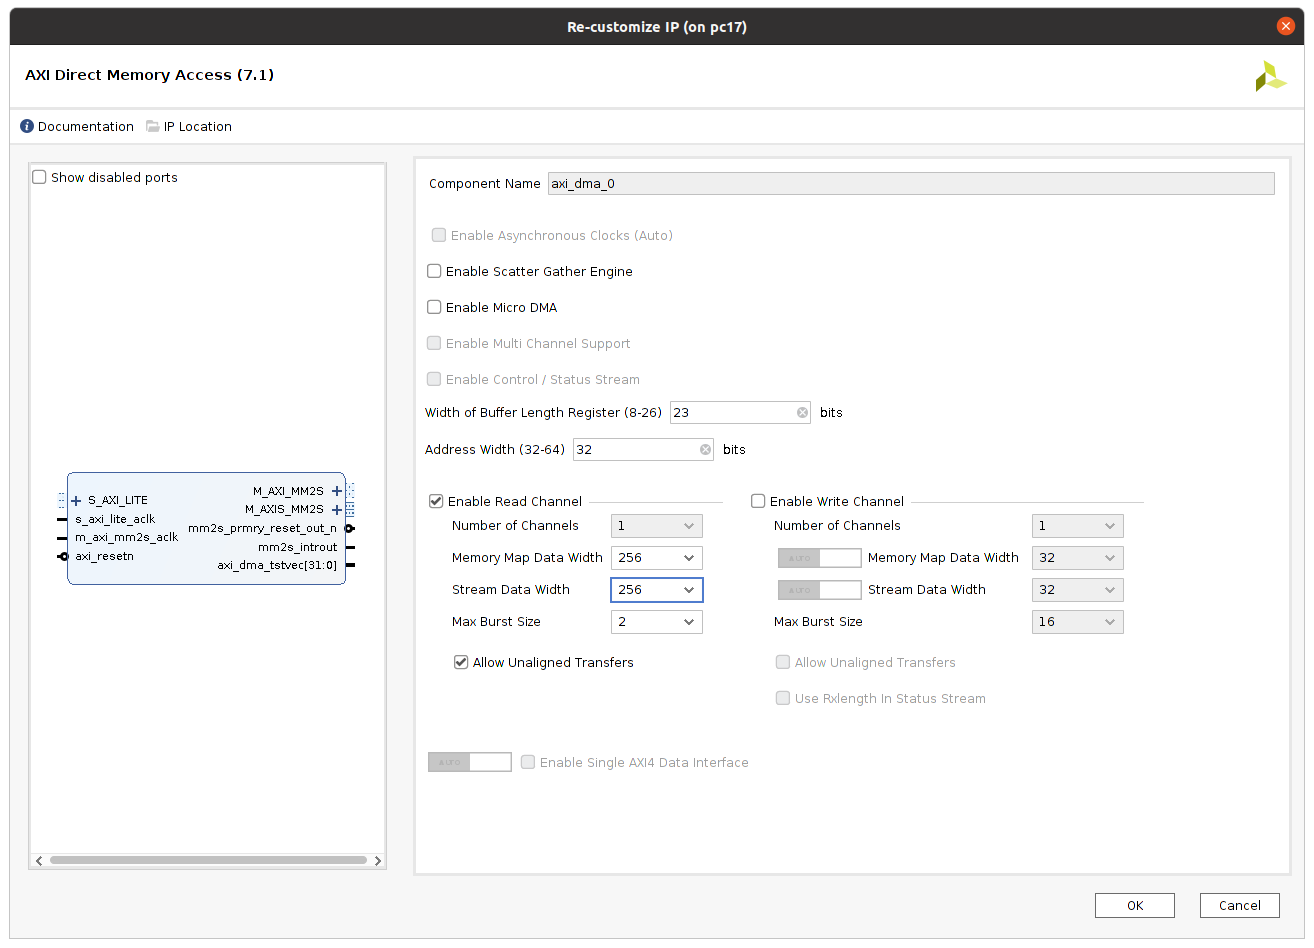
\includegraphics[scale=0.32]{images/adjust-axi-data-width.png}
\end{figure}

\subsubsection{Evaluation}

The evaluation shows that FPGA took 3.85 ms to produce the result, while CPU took 169.12 ms,
which is a 43.97x speedup.
The prediction accuracy is 88.18\%.


